\documentclass{bmcart}

%%%%%%%%%%%%%%%%%%%%%%%%%%%%%%%%%%%%%%%%%%%%%%
%%                                          %%
%% CARGA DE PAQUETES DE LATEX               %%
%%                                          %%
%%%%%%%%%%%%%%%%%%%%%%%%%%%%%%%%%%%%%%%%%%%%%%

%%% Load packages
\usepackage{amsthm,amsmath}
\usepackage{graphicx}
%\RequirePackage[numbers]{natbib}
%\RequirePackage{hyperref}
\usepackage[utf8]{inputenc} %unicode support
%\usepackage[applemac]{inputenc} %applemac support if unicode package fails
%\usepackage[latin1]{inputenc} %UNIX support if unicode package fails


%%%%%%%%%%%%%%%%%%%%%%%%%%%%%%%%%%%%%%%%%%%%%%
%%                                          %%
%% COMIENZO DEL DOCUMENTO                   %%
%%                                          %%
%%%%%%%%%%%%%%%%%%%%%%%%%%%%%%%%%%%%%%%%%%%%%%

\begin{document}

	\begin{frontmatter}
	
		\begin{fmbox}
			\dochead{Research}
			
			%%%%%%%%%%%%%%%%%%%%%%%%%%%%%%%%%%%%%%%%%%%%%%
			%% INTRODUCIR TITULO PROYECTO               %%
			%%%%%%%%%%%%%%%%%%%%%%%%%%%%%%%%%%%%%%%%%%%%%%
			
			\title{Reposicionamiento de fármacos en COVID-19}
			
			%%%%%%%%%%%%%%%%%%%%%%%%%%%%%%%%%%%%%%%%%%%%%%
			%% AUTORES. METER UNA ENTRADA AUTHOR        %%
			%% POR PERSONA                              %%
			%%%%%%%%%%%%%%%%%%%%%%%%%%%%%%%%%%%%%%%%%%%%%%
			
			\author[
			  addressref={aff1},                   % ESTA LINEA SE COPIA IGUAL PARA CADA AUTOR
			  corref={aff1},                       % ESTA LINEA SOLO DEBE TENERLA EL COORDINADOR DEL GRUPO
			  email={lauranunezj99@uma.es}   % VUESTRO CORREO ACTIVO
			]{\inits{L.N.J}\fnm{Laura} \snm{Núñez Jiménez}} % inits: INICIALES DE AUTOR, fnm: NOMBRE DE AUTOR, snm: APELLIDOS DE AUTOR
			\author[
			  addressref={aff1},
			  email={john.RS.Smith@cambridge.co.uk}
			]{\inits{I.J.P}\fnm{Inmaculada} \snm{Jiménez Palomino}}
			\author[
			  addressref={aff1},
			  email={talal.awija@gmail.com}
			]{\inits{T.A}\fnm{Talal} \snm{Awija}}
			
			%%%%%%%%%%%%%%%%%%%%%%%%%%%%%%%%%%%%%%%%%%%%%%
			%% AFILIACION. NO TOCAR                     %%
			%%%%%%%%%%%%%%%%%%%%%%%%%%%%%%%%%%%%%%%%%%%%%%
			
			\address[id=aff1]{%                           % unique id
			  \orgdiv{ETSI Informática},             % department, if any
			  \orgname{Universidad de Málaga},          % university, etc
			  \city{Málaga},                              % city
			  \cny{España}                                    % country
			}
		
		\end{fmbox}% comment this for two column layout
		
		\begin{abstractbox}
		
			\begin{abstract} % abstract
			
            A continuación, el informe trata sobre los fármacos que tienen efecto sobre las proteínas humanas que interaccionan con las 27 proteínas del Covid-19. Este caso surge debido a la pandemia vivida en nuestros días producida por el virus SARS-CoV-2, el cual está causando millones de contagios alrededor del mundo y miles de muertes. Una de las principales causas por lo que no se desarrolla de manera efectiva la creación de fármacos es por el poco conocimiento que se tiene sobre el virus. Por ello, se requiere de la búsqueda de fármacos ya existentes que puedan interaccionar con las conexiones entre proteína humana y el SARS-CoV-2, y así afectar a la reacción del virus. Nos basamos en implementar la reutilización de medicamentos basadas en la red que surge de esta relación, lo que permite clasificar todos los medicamentos aprobados en función de su posible eficacia. Usando las bases de datos STRING obtendremos dicha red, que nos ayudará a obtener las 332 proteínas humanas, las cuales, usaremos posteriormente en la base de datos de ChEMBL. Con dicha base de datos obtendremos en él, el experimento de fármacos potenciales, así como información sobre cada uno de ellos. 

 
			%%%%%%%%%%%%%%%%%%%%%%%%%%%%%%%%%%%%%%%%%%%%%%%
			%% RESUMEN BREVE DE NO MAS DE 100 PALABRAS   %%
			%%%%%%%%%%%%%%%%%%%%%%%%%%%%%%%%%%%%%%%%%%%%%%%	
			
			\end{abstract}
			
			%%%%%%%%%%%%%%%%%%%%%%%%%%%%%%%%%%%%%%%%%%%%%%
			%% PALABRAS CLAVE DEL PROYECTO              %%
			%%%%%%%%%%%%%%%%%%%%%%%%%%%%%%%%%%%%%%%%%%%%%%
			
			\begin{keyword}
			\kwd{Covid-19}
			\kwd{SARS-CoV-2}
			\kwd{ChEMBL}
			\kwd{Fármacos experimentales}
			\end{keyword}
		
		
		\end{abstractbox}
	
	\end{frontmatter}

	%%%%%%%%%%%%%%%%%%%%%%%%%%%%%%%%%
	%% COMIENZO DEL DOCUMENTO REAL %%
	%%%%%%%%%%%%%%%%%%%%%%%%%%%%%%%%%
	
	\section{Introducción}

En nuestros días estamos viviendo una pandemia que empezó en 2019 y sigue su crecimiento hasta día de hoy. El virus que originó este caos tanto económico como de salud pública mundial es el SARS-Cov-2, hallado en China a finales del año 2019. El SARS-Cov-2 tiene una alta tasa de contagios, lo que exige una actuación rápida para poder combatirlo. El virus afecta en mayor medida al sistema respiratorio, generando en cada persona diferentes grados de síntomas o en algunos casos hasta la muerte. Aunque, también se ha encontrado que el virus afecta a diferentes tejidos del cuerpo. Debido al gran impacto que ha generado en el mundo en todos los ámbitos, se necesita de manera urgente encontrar vacunas o medicamentos. 

\begin{figure}[h!]
			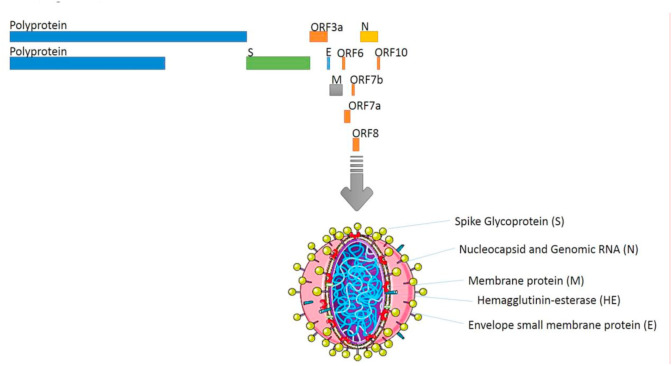
\includegraphics[width=0.9\textwidth]{figures/gr1_lrg.jpg}
			\caption{Estructura del coronavirus}
			\label{fig:cost_genome}
		\end{figure}
\newpage
		
Para la reutilización de medicamentos o de la creación de nuevos medicamentos, se necesita saber como actúa el SARS-CoV-2 durante la infección y los cambios moleculares en las proteínas humanas. Hoy en día, no hay medicamentos antivirales contra el coronavirus. Dicho anteriormente, el desconocimiento de detalles de la molécula del SARS-Cov-2, impide que se obtenga una evaluación precisa para la creación de fármacos. Esto supone un largo tiempo de investigación.

Después de ver unos cuantos artículos sobre como resuelven este problema de la reutilización del fármaco, concluimos en que la mejor estrategia es la basada en la elección de fármacos a través de la creación de una red interactoma humano perturbado por el SARS-Cov-2. A partir de ella, se verá los tejidos afectados por el virus y se priorizará los medicamentos existentes en función de las proteínas humanas y dichas interacciones. Para interrumpir el interactoma del SARS-CoV-2, buscamos ligandos de proteínas humanas que interactúen con proteínas virales. 

		

	\section{Materiales y métodos}

En este apartado se explicará los diferentes métodos que se han seguido a lo largo de un proceso para la reutilización de fármacos.

El inicio de nuestra investigación se ha basado leyendo un número de artículos para ponernos en situación del virus SARS-CoV-2. Encontramos en unos de los paper \cite{Gordon2020}, que el virus forma 29 proteínas, pero que tan solo han sido clonadas y expresadas 26 proteínas de las 29.  Estas 26, las señaladas en la tabla 1, son las usada en la investigación y con las que será generado el interactoma proteínas humanas-SARS-Cov-2. 


\subsection{STRING, Protein-Protein Interaction Networks}

Visto anteriormente, la principal idea es obtener que relaciones tienen las proteínas del virus con nuestro cuerpo. De esta manera, sabremos con que proteínas humanas interactúan y así encontrar fármacos que afecten directamente a ellas. El pensamiento es que estos fármacos eviten en cierta medida, la clonación y la infección del virus de manera indirecta. 

Para encontrar las proteínas secundarias, llamadas de esta forma en los artículos leídos, se hará uso de la base de datos STRING. 
STRING se usa para obtener las relaciones de las proteínas del SARS-Cov-2, con todas las humanas. Las proteínas humanas mostradas en STRING son 332 que serán clave en la investigación de los fármacos. 

\subsection{redSring.R}

Una vez hecho la búsqueda de las 332 proteínas humanas, las guardamos en un fichero de entrada. Posteriormente este archivo, creará un mapeo de estas mismas proteínas, pero queriendo reducir el número de ellas. 

El archivo ejecutará un mapeo sobre las 332 proteínas humanas encontradas en STRING. Utilizará el fichero donde vienen las proteínas y creará un dataframe donde vendrán el nombre de las proteínas y además se añadirá una columna con STRINGID de cada una de ellas. Después, la intención es obtener una subred de las interacciones entre esas 332, para generar una red secundaria de las interacciones más fuertes. Para ello hemos utilizado un combined score mayor a 900. 

Este proceso se utiliza, porque nos ayudará a tener unos resultados más fiables a la hora de encontrar fármacos. Debido a que encontraremos fármacos que afecten a relaciones muy estrechas. 

\subsection{convertirUniprot.R}

Este fichero es auxiliar. Nos va a ayudar a convertir los Gene Name de las proteinas obtenidas en el archivo redString.R, en su nombre de UniProt. Por lo que, devolverá un fichero .txt con los respectivos nombres. 

Se realiza esta conversión, para tener los datos preparados en la búsqueda de fármacos en CHEMBL. 

\subsection{Bases de datos CHEMBL y fichero consultarChembl.py}

    \subsubsection{Bases de datos CHEMBL y consultas en Myqsl}
    En el informe de la explicación de la práctica, nos dice que: Las proteínas humanas con las que interaccionan las proteínas virales de SARSCoV2 pueden ser targets farmacológicos de interés, por lo que en este proyecto se pretende encontrar fármacos de la base de datos ChEMBL que tengan como diana las proteínas o módulos del interactoma funcional SARS-humano. Por lo tanto, todo lo que se ha hecho hasta ahora es facilitar el trabajo para que una vez hayamos obtenidos esos denominados targets, se busquen en esta bases de datos. 
    
    ChEMBL tiene la posibilidad de ser descargada en diferentes formatos para ser trabajada desde Oracle, MySQL, XML, etc. La base de datos ChEMBL ha sido descargada en formato MySQL para realización del informe. Mediante un esquema de las tablas proporcionadas y una guía donde explica cada tabla y cada elemento, hemos podido hacer la consulta sobre los fármacos que queremos. Hemos realizado una ruta entre las tablas que necesitamos acordes con los datos preparados. 
    
    La consulta en cuestión es: 
    
		\begin{figure}[h!]
			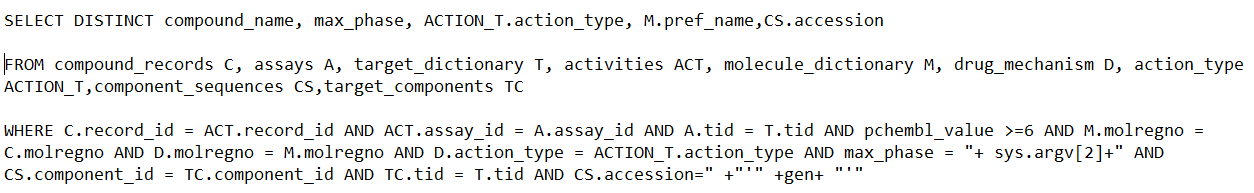
\includegraphics[width=0.9\textwidth]{figures/Captura.PNG}
			\caption{Consulta MySQL}
			\label{fig:cost_megabase}
		\end{figure}
	\newpage
		
	Tal y como podemos ver en esta consulta, accedemos a varias tablas de la base de datos. Para explicar esto mejor, vamos a mostrar el esquema de la base de datos de Chembl, pero únicamente las tablas que hemos utilizado:
    
    \begin{figure}[h!]
			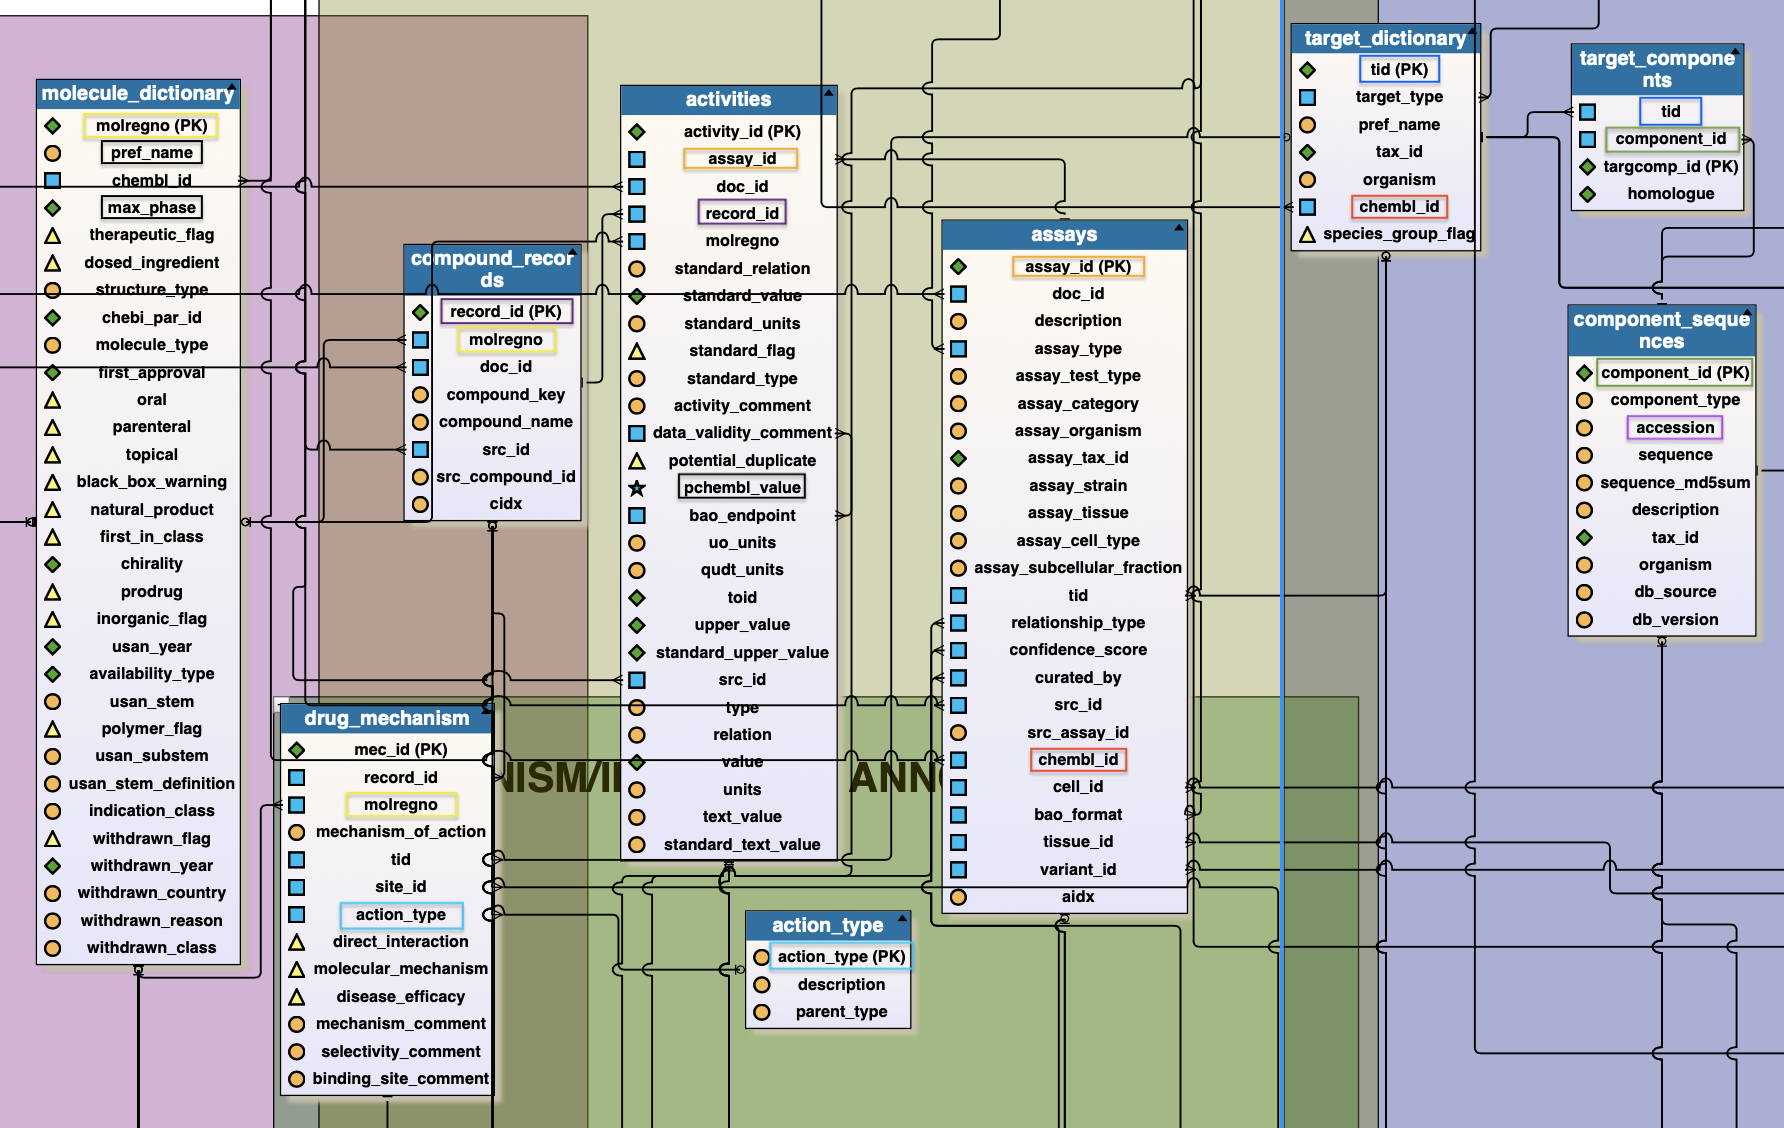
\includegraphics[width=0.9\textwidth]{figures/esquema.png}
			\caption{Esquema Chembl DB}
			\label{fig:cost_megabase}
		\end{figure}
	
    Accedemos a este esquema por el atributo \textbf{accession} de la tabla \textbf{component sequences}, en las que introducimos el UniprotID de las 178 proteínas humanas que hemos extraído anteriormente.  
    
    Desde ahí, recorremos un camino, marcado en la figura con recuadros en los atributos de cada tabla, en el que pasamos por la tabla \textbf{target components} a través del component id de la proteínas, cogemos el tid y llegamos a la tabla \textbf{target dictionary}, de donde sacaremos el Chembl ID de la proteína para llegar a la tabla \textbf{assays}.  
    
    Con el assay id accedemos a la tabla \textbf{activities}, que además de formar parte de la ruta desde la proteína hasta sus fármacos asociados, contiene el valor de P Chembl, que vamos a utilizar para filtrar los fármacos: con un P Chembl value mayor a 6 nos aseguramos que los compuestos estén estrechamente relacionados con las proteínas. En esta misma tabla, nos encontramos el record id, que nos servirá para enlazar con la tabla \textbf{compound records}, nuestro objetivo. 
    
    Una vez llegados aquí, ya tenemos la lista de fármacos asociados, pero hemos indagado más, recurriendo a las tablas \textbf{molecule dictionary}, \textbf{drug mechanism} y \textbf{action type} para incluir en nuestra consulta, además, el tipo de acción que ejerce el fármaco, la fase de ensayo en la que se encuentra (que hemos dividido en fármacos experimentañes, fase 3, y fármacos aprobados, fase 4) y el nombre común que tienen los compuestos, ya que el científico resultaba muy poco evidente.
    
    
    \subsubsection{Código en python. consultarChembl.py}
    Debido al gran número de proteínas obtenidas, sería muy costoso y lento ir buscando en la consulta de MySQL una a una. Por lo que, se ha creado un programa Python, que lee el fichero donde se encuentran las 178 proteínas con sus respectivos nombres y UniProt ID.
    
    El programa se conecta a las bases de datos descargada en el ordenador y procede a hacer un bucle leyendo cada línea del fichero. De esta manera, va leyendo cada UniProt ID y la va introduciendo en la consulta para ir obteniendo nuestro resultado final que sería los fármacos que estábamos buscando al inicio de la investigación. 
    
    Se ha decidido que los fármacos buscados sean del tipo 3 y 4. Donde el tipo 3 son fármacos experimentales y de tipo 4 fármacos aprobados. Esta decisión es debida a que así tendremos una certeza adecuada de funcionalidad del fármaco hallado. 

    
    
\subsection{analisisResultados.R}
La ejecución de este fichero sirve para obtener graficas sobre los fármacos encontrados y poder evaluar los resultados obtenidos. 
El arvicho que recoge el fichero es el obtenido en el programa de Python. 

\subsection{launch.sh}
Es un flujo del trabajo completo, el fichero que hay que ejecutar para que se lleve a cabo todo el proceso. Es el fichero principal, un flujo bash


	
\section{Resultados}
Tras ejecutar todos los pasos, todos los resultados obtenidos se irán guardando en la carpeta results. Como se han seguido una serie de pasos durante la investigación, en este apartado se irán mostrando los resultados de cada sección. 

Antes de hacer la investigación, leímos varios artículos para encontrar el número de proteínas del SARS-CoV-2. Las proteínas encontradas fueron las mostradas en la tabla. 

  

		\begin{table}[h!]
			\caption{Proteinas del SARS-CoV-2 usadas en la red}
			\begin{tabular}{cccc}
				\hline
				& Proteínas del covid  &   & \\ 
				\hline
				"NSP6" & "NSP1" & "NSP2" & "NSP5"\\
				"NSP7" & "NSP5" & "NSP8"  & "NSP9"\\
				"NSP11" & "NSP12" & "NSP13" & "NSP14"\\ 
				"NSP15" & "S" & "E" & "N"\\
				"M" & "ORF3a" & "ORF3b" & "ORF8"\\
				"ORF6" & "ORF7a" & "ORF9b" & "ORF9c"\\
                "ORF10" \\
				\hline
				\label{tab:ejemplo}
			\end{tabular}
		\end{table}

		
En los artículos venían que había 29 proteínas, pero que solo se utilizaron 26 de ellas. Por eso en los resultados, sólo hay 26. 
El fichero que contienen las proteínas las introducimos en STRING para encontrar el interactoma y tuvimos de resultado la siguiente red. 

		\begin{figure}[h!]
			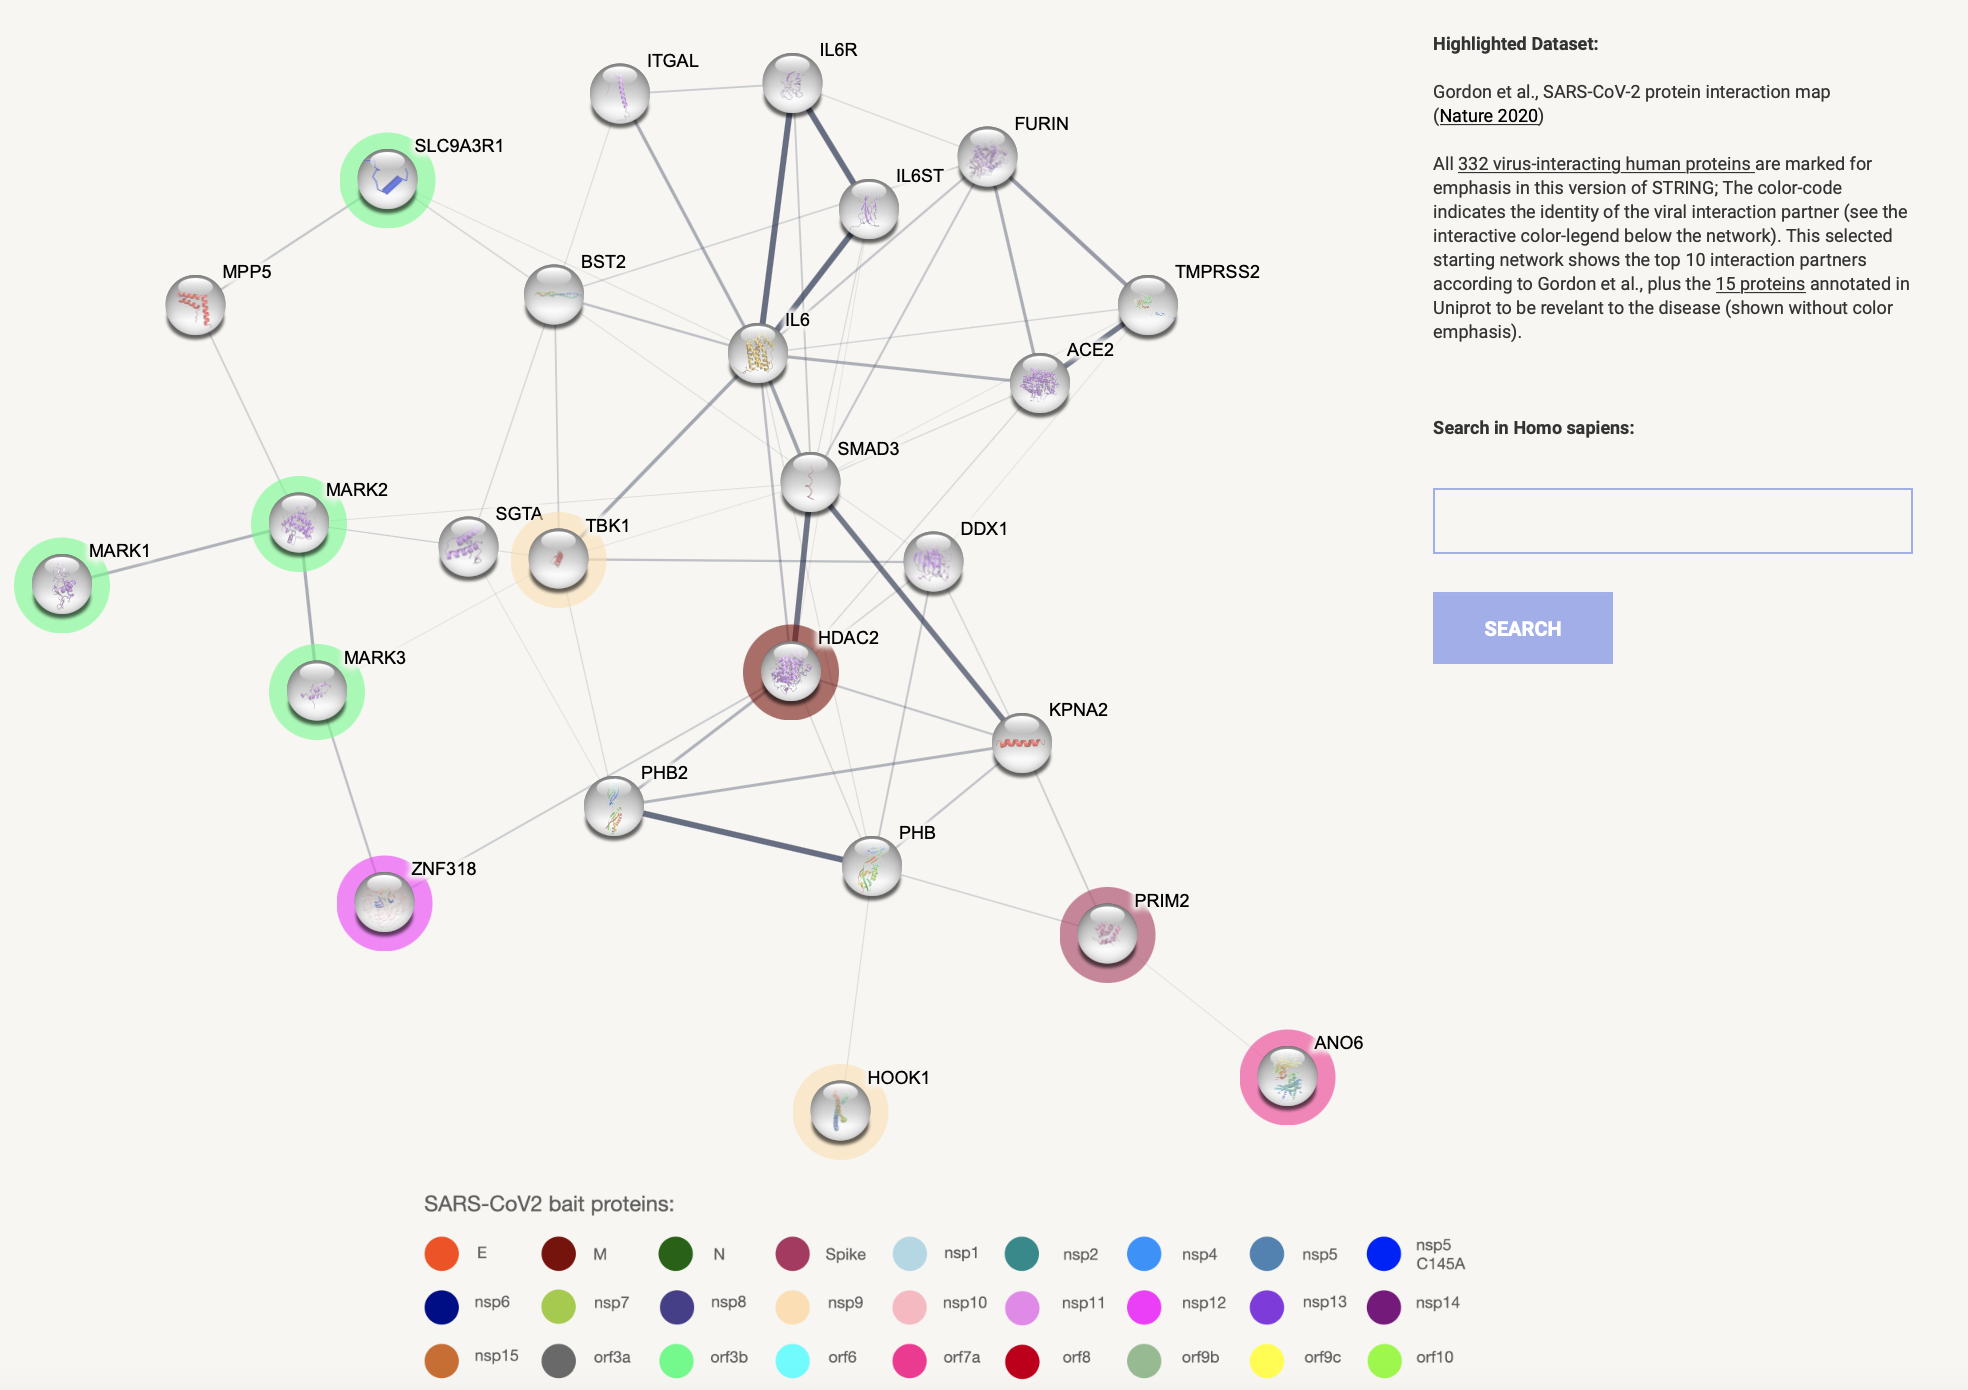
\includegraphics[width=0.8\textwidth]{figures/redinteractoma.jpg}
			\caption{Red proteinas humanas-proteinas SARS-CoV-2}
			\label{fig:cost_megabase}
		\end{figure}
		


En STRING obtuvimos 332 proteínas que interactuaban con las proteínas del SARS-CoV-2. Pero la red se divide en varios módulos, porque cada proteína del SARS-CoV-2 interactúa con un numero X de proteínas humanas. Por lo que, descargamos las 332 proteínas humanas para crear posteriormente una red entre ellas y elegir las que más fuerza de interacción tengan. 

Ejecutamos el fichero redString y nos da el resultado de 178 proteínas secundarias, que son las que usaremos para la búsqueda de los fármacos. 

		\begin{figure}[h!]
			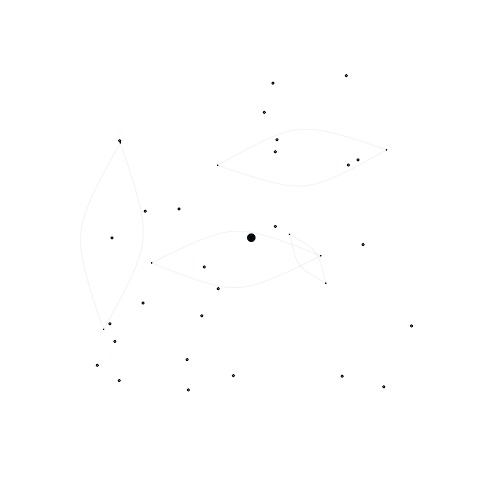
\includegraphics[width=0.6\textwidth]{figures/redsecundaria.jpeg}
			\caption{Red de proteinas huamnas}
			\label{fig:cost_megabase}
		\end{figure}
		
	\newpage

Todas esos genenames de proteinas las pasamos a Uniprot ID. 
		\begin{figure}[h!]
			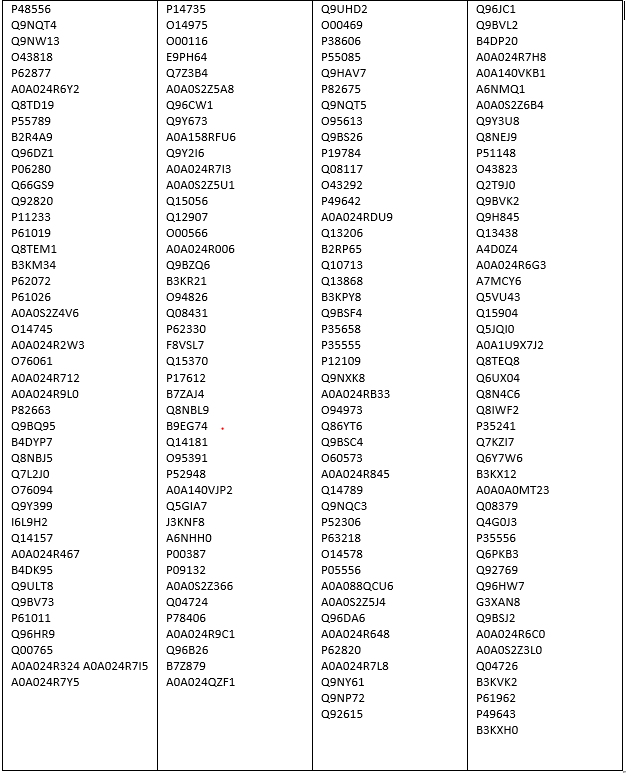
\includegraphics[width=0.9\textwidth]{figures/Captura1.PNG}
			\caption{Uniprot ID de las proteínas obtenidas en la red}
			\label{fig:cost_megabase}
		\end{figure}
		
Una vez obtenidos los UnitProt ID, buscamos los fármacos en la base de datos ChEMBL. Tras obtener loas datos de los fármacos tanto para la fase de aprobación como para la experimental, se realiza una serie de gráficos. A continuación, vamos a mostrar dos gráficas, una donde serán los tipos de fármacos que se utilizan en ensayos ya aprobados y la otra grafica los tipos de los ensayos experimentales. 

Se obtienen alrededor de 43 fármacos de ensayos experimentales y unos 66 de fármacos en los ensayos aprobados. 

\newpage

		\begin{figure}[h!]
			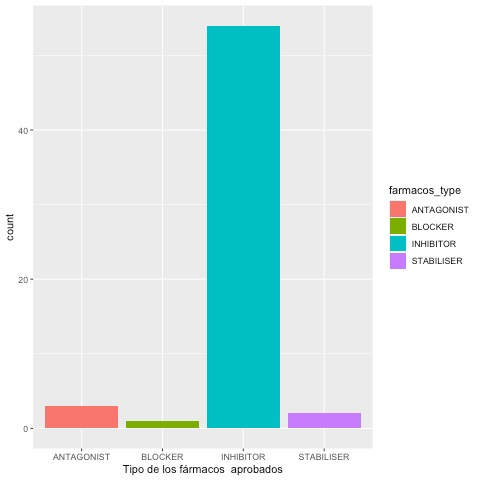
\includegraphics[width=0.7\textwidth]{figures/farmacosaprobados.jpeg}
			\caption{Grafica del tipo de fármacos aprobados}
			\label{fig:cost_megabase}
		\end{figure}
 


		\begin{figure}[h!]
			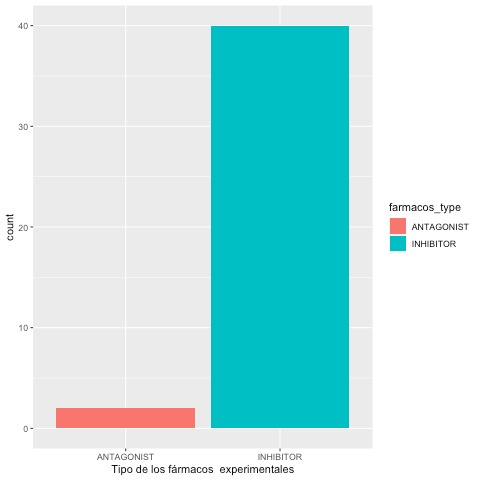
\includegraphics[width=0.7\textwidth]{figures/farmacosexperimentales.jpeg}
			\caption{Grafica del tipo de fármacos aprobados}
			\label{fig:cost_megabase}
		\end{figure}
Como observamos en esta primera grafica y en la segunda, la mayor parte de fármacos son de tipo inhibidor.

\newpage
	\section{Discusión}
Lo más destacable de los resultados es que, el tipo de fármaco que predomina sobre todos son los inhibidores, que disminuyen o cesan la acción o creación de otra sustancia. 

Nos podemos imaginar y deduciendo de los artículos leídos \cite{Gordon2020} \cite{Gysi2020} \cite{Sayed2020} que los fármacos pueden bloquear, en cierto modo, que las células del SARS-CoV-2 invadan las células humanas o limitar entres proceso que causa la infección. De esta manera, los síntomas y el tiempo de la enfermedad se podrían ver limitados. 

Todo lo desarrollado es en general, permite que se puedan buscar fármacos en otras fases de ensayos y especificar más que realiza cada fármaco. Por lo que, no solo existen los fármacos de nuestra lista. 
	\section{Conclusiones}
Finalmente, el objetivo que teníamos al inicio de la investigación de encontrar fármacos que puedan actuar sobre el virus del SARS-CoV-2 usando la base de datos ChEMBL ha sido completada. Al inicio del trabajo creamos el interactoma de las proteínas, pero debido a que hay muchos módulos dentro de ese mismo interactoma, es difícil encontrar un interactoma funcional completo. Otro dato, es que al hacer el mapeo solo se pierden la mitad casi de las proteínas, es decir, tenemos un alto nivel de interacción entre bastantes proteínas secundarias, por lo que será de mayor ayuda en la búsqueda de los fármacos, ya que saldrán resultados más certeros. Aun así, nos sale de resultados un gran número de fármacos ya aprobados. Además, dentro de estos fármacos podemos observar, que se encuentran un mecanismo de acción mayoritario, es el caso de fármacos inhibidoras. Como consecuencia de todo podemos concluir que hay que estudiar qué proteínas del interactoma funcional son las mejores candidatas que desarrollar un fármaco.  

	
	
	%%%%%%%%%%%%%%%%%%%%%%%%%%%%%%%%%%%%%%%%%%%%%%
	%% OTRA INFORMACIÓN                         %%
	%%%%%%%%%%%%%%%%%%%%%%%%%%%%%%%%%%%%%%%%%%%%%%
	
	\begin{backmatter}
		
		\section*{Disponibilidad de datos y materiales}%% if any
			https://github.com/talal314/project_template.git
		
		\section*{Contribución de los autores}
			T.A:Uso y descarga de la base de datos ChEMBL,consultas y recorrido de tablas sobre la bases de datos, Connectar a la base de datos desde python para guardar los resultados en una tabla y filtración de datos con R. 
			
			I.J.P: Obtención de las proteinas humanas, creación de igraph y mapeo de dichas proteínas, filtración de las interacciones con combined score y transformación del id a uniprot id. 
			
			L.N.J: Redacción del informe de la investigación. Consultar y buscar información en artículos y la obtención de las 29 proteínas del SARS-CoV-2. 
		
		
		%%%%%%%%%%%%%%%%%%%%%%%%%%%%%%%%%%%%%%%%%%%%%%%%%%%%%%%%%%%%%%%%%%%%%%%%%%%%%%%%%%%%%%%%
		%% BIBLIOGRAFIA: no teneis que tocar nada, solo sustituir el archivo bibliography.bib %%
		%% por el que hayais generado vosotros                                                %%
		%%%%%%%%%%%%%%%%%%%%%%%%%%%%%%%%%%%%%%%%%%%%%%%%%%%%%%%%%%%%%%%%%%%%%%%%%%%%%%%%%%%%%%%%
		
		\bibliographystyle{bmc-mathphys} % Style BST file (bmc-mathphys, vancouver, spbasic).
		\bibliography{library}      % Bibliography file (usually '*.bib' )
	
	\end{backmatter}
\end{document}
